\section{Discussion}


\begin{comment}
Is any of this useful to mention here?

\subsection{Transiting Exoplanet Survey Satellite (TESS)} \label{sec:TESS}

\begin{figure}[h]
    \centering
    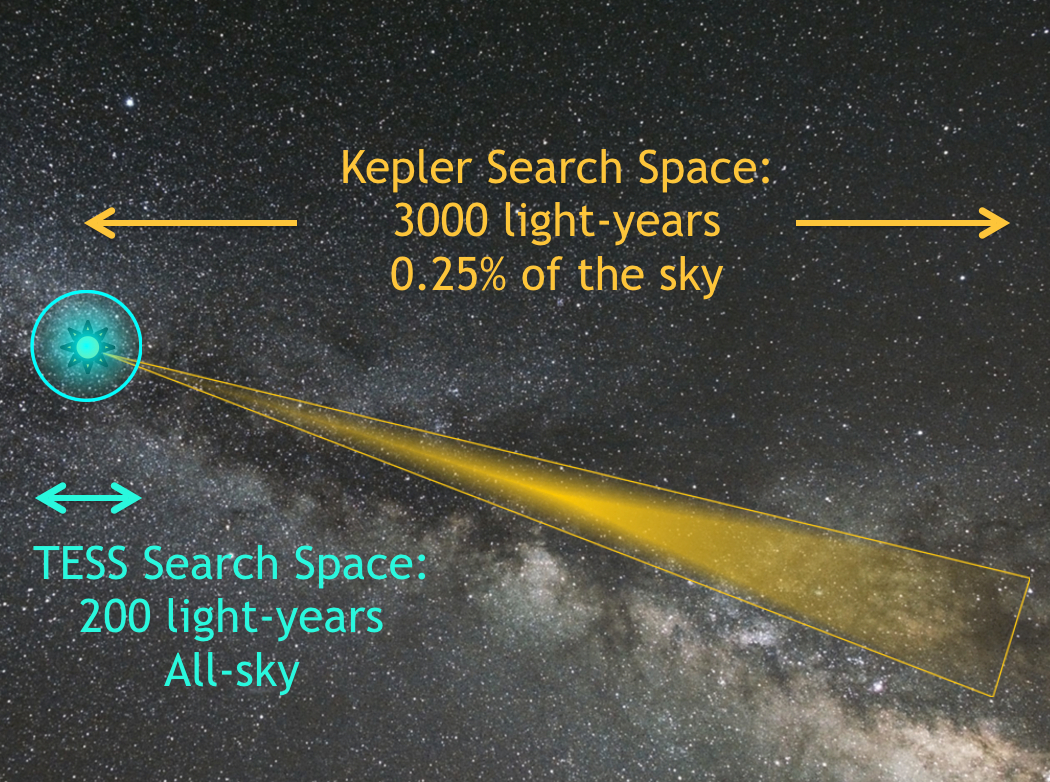
\includegraphics[width=0.9\linewidth]{figures/images/TESS_vs_Kepler}
    \caption{Comparison of the survey strategies of the \textit{Kepler} and TESS missions\protect\footnotemark[4]{}. \textit{Kepler} focused on a deep search of a small region of the sky, while TESS conducts a wide-field survey targeting nearby stars across nearly the entire sky.}
    \label{fig:TESS_vs_Kepler}
\end{figure}

\footnotetext[4]{\url{https://www.nasa.gov/space-science-and-astrobiology-at-ames/division-overview/astrophysics-branch-overview-sta/exoplanet-mission/exoplanet-research-projects}}

Following the success of the \textit{Kepler} and K2 missions, NASA launched the Transiting Exoplanet Survey Satellite (TESS) to carry out a wide-field survey of nearly the entire sky, focusing on nearby, bright stars well suited for follow-up characterization \citep{Ricker2015, Huang2018}. This observing strategy puts emphasis on short-period planets orbiting luminous host stars which are better suited for precision mass measurements and atmospheric studies.

TESS monitors the sky in sectors with typical observing baselines of $\sim27$ days each. Compared to \textit{Kepler}, which maintained continuous observations of the same field, this is significantly shorter. Figure~\ref{fig:TESS_vs_Kepler} shows an artist rendition of the field of view covered by TESS in comparison to that of \textit{Kepler}. As a result, TESS is most sensitive to planets with orbital periods shorter than $\sim10$–$20$ days. Longer period planets remain better constrained by the extended \textit{Kepler} dataset \citep{Sullivan2015}. Despite this limitation, TESS has greatly expanded the known population of transiting exoplanets and produced thousands of candidates orbiting bright nearby stars across the sky \citep{Guerrero2021}.

Together, \textit{Kepler} and TESS complement one another on insights into exoplanet populations. The long baseline and high photometric precision of \textit{Kepler} allowed for statistical studies of population occurrence rates and structure. One prominent result is the discovery of the “radius valley”, a deficit of planets with radii around $1.5$–$2R_{\oplus}$ that separates two dominant populations of super-Earths and sub-Neptunes \citep{2017AJ....154..109F, 2018MNRAS.479.4786V}. In contrast, TESS primarily detects planets orbiting bright nearby stars, making these systems well suited for detailed follow-up observations. These include radial velocity mass measurements and atmospheric characterization with facilities such as the James Webb Space Telescope. TESS is the connection between the statistical studies of exoplanet populations and parameter estimation of planetary systems \citep{Batalha2019}.

\subsection{PLAnetary Transits and Oscillations of stars (PLATO)} \label{sec:PLATO}

Looking ahead, the European Space Agency (ESA) is preparing the next major mission in exoplanet transit research. Known as the \textit{PLAnetary Transits and Oscillations of stars} (PLATO) mission, its objective is to extend the work \textit{Kepler} and TESS by introducing high-precision, long-baseline photometric monitoring of bright stars across large areas of the sky \citep{Rauer2014}. The mission is currently scheduled to launch between late 2026 and early 2027. PLATO's primary goal is to detect and characterize terrestrial exoplanets orbiting within the habitable zones of their host stars. Furthermore, the mission will perform asteroseisomology to determine precise stellar ages, radii, and masses.

PLATO will combine wide-field coverage with long-duration observations lasting several years in selected fields. In contrast to TESS, PLATO's strategy is optimized for detecting small planets with longer orbital periods which are much more difficult to observe with current all-sky transit surveys \citep{Rauer2014}. The mission is expected to produce a statistically robust sample of Earth-sized planets with well constrained host-star properties. Such measurements will enable detailed study of planetary system evolution and improve estimates of habitable worlds in the solar neighbourhood. 

Together, PLATO, \textit{Kepler}, and TESS form a complementary sequence of transit surveys. Collectively, they span deep narrow-field observations, all-sky coverage of bright stars, and future baseline characterization of nearby terrestrial systems.  Within this progression, PLATO is anticipated to provide the precise stellar and planetary parameters necessary to connect statistical exoplanet demographics with detailed physical characterization \citep{PLATO2022}.
\end{comment}